\documentclass[tikz,border=12pt]{standalone}
\usetikzlibrary{arrows.meta,positioning,calc}

\begin{document}
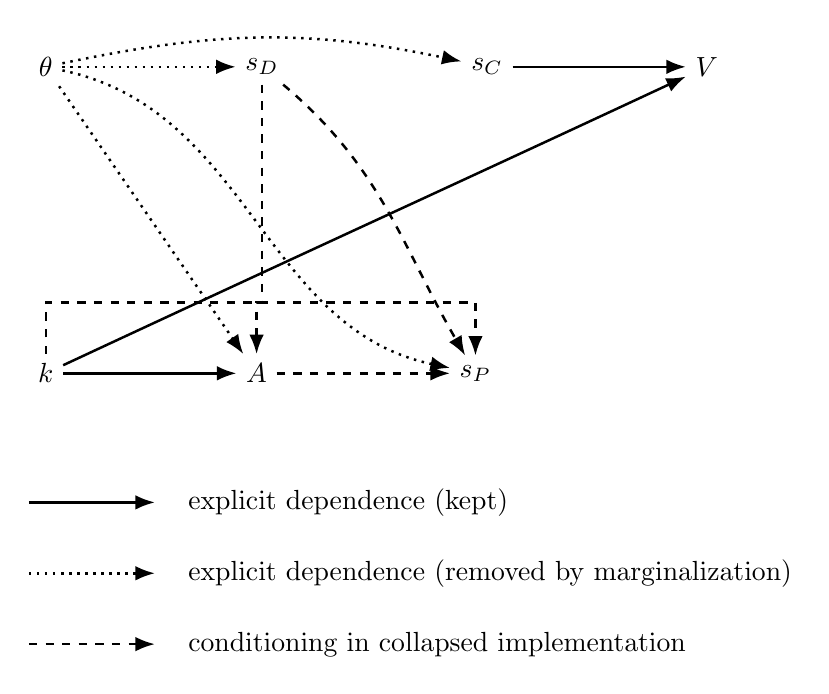
\begin{tikzpicture}[
  >=Latex,
  node distance=3.4cm and 2.2cm,
  every node/.style={align=center},
  solidedge/.style={-Latex, line width=0.9pt},
  dashededge/.style={-Latex, dashed, line width=0.9pt},
  dottededge/.style={-Latex, dotted, line width=0.9pt}
]

% --- Layout
\node (theta) {$\theta$};
\node[right=of theta] (sD) {$s_D$};
\node[right=of sD]    (sC) {$s_C$};
\node[right=of sC]    (V)  {$V$};

\node[below=of theta] (k) {$k$};
\node[right=of k]     (A) {$A$};
\node[right=of A]     (sP) {$s_P$};

% --- Solid edges (kept in both)
\draw[solidedge] (k) -- (A);
\draw[solidedge] (sC) -- (V);
\draw[solidedge] (k) to[out=25,in=205] (V);

% --- Dotted edges (removed in collapsed tree)
\draw[dottededge] (theta) -- (sD);
\draw[dottededge] (theta) to[out=12,in=168] (sC);
\draw[dottededge] (theta) -- (A);
\draw[dottededge] (theta) to[out=-12,in=168] (sP);

% --- Dashed edges (conditioning added in collapsed tree)
\draw[dashededge] (sD) to[out=-40,in=120] (sP);
\draw[dashededge] (A) -- (sP);
\draw[dashededge] (k) |- ($(A)+(0,0.9)$) -| (sP);
\draw[dashededge] (sD) |- ($(A)+(0,0.9)$) -| (A);

% --- Legend below diagram
\coordinate (sw) at (current bounding box.south west);
\draw[solidedge] ($(sw)+(0,-1.4)$) -- +(1.6,0);
\node[anchor=west] at ($(sw)+(1.9,-1.4)$) {explicit dependence (kept)};
\draw[dottededge] ($(sw)+(0,-2.3)$) -- +(1.6,0);
\node[anchor=west] at ($(sw)+(1.9,-2.3)$) {explicit dependence (removed by marginalization)};
\draw[dashededge] ($(sw)+(0,-3.2)$) -- +(1.6,0);
\node[anchor=west] at ($(sw)+(1.9,-3.2)$) {conditioning in collapsed implementation};

\end{tikzpicture}
\end{document}
